\documentclass[aps,prresearch,reprint,amsmath,amssymb,longbibliography,floatfix]{revtex4-2}

\usepackage[utf8]{inputenc}
\usepackage[T1]{fontenc}
\usepackage{booktabs}
\usepackage{graphicx}
\graphicspath{{outputs/figures/}}
\usepackage{xcolor}
\usepackage{hyperref}

\hypersetup{colorlinks=true,linkcolor=blue!60!black,
            citecolor=blue!60!black,urlcolor=blue!60!black}

\newcommand{\Fi}{F_i}
\newcommand{\nop}{\hat{n}}
\newcommand{\adag}{\hat{a}^\dagger}
\newcommand{\aop}{\hat{a}}
\newcommand{\rhohat}{\hat{\rho}}
\newcommand{\Lop}{\hat{L}}

\begin{document}

\title{Local number variance as a redistribution handle in the one-dimensional Bose--Hubbard chain}

\author{Kunal Bhatia}
\email{kunal29bhatia@gmail.com}
\affiliation{Independent Researcher, Heidelberg, Germany}
\altaffiliation{ORCID: \href{https://orcid.org/0009-0007-4447-6325}{0009-0007-4447-6325}}

\date{\today}

\begin{abstract}
We test whether the local occupation variance
$\Fi = \langle\nop_i^2\rangle - \langle\nop_i\rangle^2$ identifies
intervention subsets with enhanced finite-horizon response in a
one-dimensional open Bose--Hubbard chain under Lindblad dephasing.
Additional dephasing at the top-$k$ highest-$\Fi$ sites is compared
against matched-budget random targeting across 100 independent trials
per condition, using exact Lindblad evolution in the fixed-particle-number
sector ($L\in\{6,7,8\}$, $\tau\in\{1,2,3\}$).
The primary sweep reveals three regimes: at $J/U=0.12$ the response is
near-zero to weakly harmful (95\% CI below zero at the paper's burn-in
time, but small in magnitude and partly burn-in-sensitive at $L=6$);
near $J/U\approx0.20$ there is a crossover that is sensitive to system size
and horizon; at $J/U\geq0.30$ targeted intervention is reliably
\emph{beneficial} (CI above zero at every tested $(L,\tau)$ combination),
with best effects at $J/U=0.40$, $\tau=3$: $+0.047$ ($L=6$), $+0.068$
($L=7$), $+0.072$ ($L=8$).
To disentangle variance information from geometry, we perform four
additional experiments.
A disorder selector sweep ($L=6$, 50 realizations, 9 selectors) at strong
disorder ($\mu_{\max}\geq1.0$) shows that $\Fi$ is the top selector,
ranking above geometric centrality (geo), mean occupation (maxn/minn),
disorder amplitude (dis\_amp), and a generator-action selector (gen); the
$\Fi$--geo gap grows monotonically with disorder strength and $J/U$,
confirming that $\Fi$ carries information beyond raw spatial position.
Shell-matched permutation controls ($L=6$, $\mu_{\max}\leq0.3$) show that
$\Fi$ beats all within-shell permutations by $+0.002$--$+0.006$ at
$\tau=3$, $J/U\geq0.30$, establishing that the advantage is not reducible
to shell geometry.
A deterministic inhomogeneous tilt chain ($L=6$) where $\Fi\neq\mathrm{geo}$
by construction gives $\Fi>\mathrm{geo}$ with a gap of $+0.032$--$+0.054$
at $J/U=0.40$, $\tau=3$, confirming the result under designed symmetry
breaking.
A scan of the extra dephasing rate ($\gamma_{\mathrm{extra}}\in
\{0.1,0.2,0.5,1.0,2.0\}$) shows the advantage peaks near
$\gamma_{\mathrm{extra}}=0.5$--$1.0$ and collapses at very high rates,
confirming that the paper's choice $\gamma_{\mathrm{extra}}=0.5$ is
near-optimal.
Taken together, local number variance functions as a finite-size,
regime-dependent redistribution handle in the positive pocket
($J/U\geq0.30$): it identifies intervention subsets with enhanced
finite-horizon response, and this advantage is not reducible to geometric
centrality, shell position, mean occupation, or disorder amplitude, while
surviving the tested deterministic symmetry-breaking controls.
Because the systems are small enough for exhaustive enumeration, we further
rank the $\Fi$-selected subset against all $\binom{L}{k}$ possible
intervention subsets: in the positive-pocket regime it lies at the top of
the subset-response distribution at every tested $(L,\tau)$ pair, and the
conclusion survives signed, absolute, and redistribution-based target
definitions.
Finite-difference susceptibility analysis shows that $\Fi$ is not a
local-depletion susceptibility but a redistribution susceptibility:
Spearman$(\Fi,\chi^{\mathrm{redist}})$ is positive across all regimes and
all horizons, and the top-$\Fi$ sites exactly match the highest
redistribution-susceptibility sites at $L=6$, $\tau\geq2$.
We further apply pre-registered structural analyses to the same
simulation data. Across all 52 saved $(L,J/U,\tau)$ cells, the
pre-intervention site that best predicts the random-arm response
disagrees with the site of largest causal advantage in $90.4\%$ of
cells, identifying predictive observability and intervention leverage
as structurally distinct channels. At $L=8$, the principal direction of
the per-site response in site space reorients sharply across
$J/U=0.30$, with threshold-vs-off-threshold direction-angle ratio
$3.25\times$ under the redistribution-gap observable, supplying a
structural correlate of the empirical regime boundary; at $L=9$ the
same signature is not visible within the available simulations.
Three further structural results---subspace clustering of observables
by physical class (KS $p<10^{-5}$ versus a uniform-Stiefel null at every
$L$), thermalization-driven convergence of observable subspaces (median
pairwise principal angle at $L=6$: $1.40$ rad at $\tau=1$, $0.18$ rad
at $\tau=3$), and $100\%$ cell-level disagreement of three natural
single-site scoring rules---are reported as supporting findings, with
two pre-registered numerical predictions reported as failed to bound
the structural reach honestly.
\end{abstract}

\maketitle

\section{Introduction}
\label{sec:intro}

The one-dimensional Bose--Hubbard model is a standard setting for studying
the interplay of quantum tunnelling and on-site interactions in interacting
boson systems~\cite{fisher1989,jaksch1998}.
At zero temperature the model exhibits a quantum phase transition between a
superfluid phase (large $J/U$) and a Mott-insulating phase (small $J/U$),
controlled by the ratio of tunnelling amplitude~$J$ to on-site
interaction~$U$~\cite{kuhner2000,greiner2002}.
The clean-system phase diagram and its experimental realisation in
optical lattices~\cite{jaksch2005} have been extensively
studied~\cite{greiner2002}.

In the presence of dissipation---modelled by local dephasing in the
Lindblad--Gorini--Kossakowski--Sudarshan (LGKS)
framework~\cite{lindblad1976,gorini1976,breuer2002}---the system is
driven away from the ground state and develops spatially heterogeneous
fluctuation structure.
Open quantum systems of this type arise naturally in cold-atom experiments
where coupling to photon-field fluctuations causes local dephasing of
on-site number states~\cite{pichler2010,poletti2012}.
More broadly, the engineering of dissipation as a resource for state
preparation and quantum control has attracted significant theoretical and
experimental attention~\cite{diehl2008,verstraete2009,sieberer2016,daley2014}.

A natural question in any driven-dissipative system is whether local
structural variables can serve as targeted control handles: does
selectively perturbing sites identified by a local observable produce
measurably different future outcomes than applying the same perturbation
budget at randomly chosen sites?
In open quantum systems governed by a Lindblad master equation this
question has received little direct quantitative attention.

This paper tests one specific instance.
Under uniform dephasing, sites in the Bose--Hubbard chain develop different
local occupation variances $\Fi = \langle\nop_i^2\rangle -
\langle\nop_i\rangle^2$, reflecting the degree of local number
fluctuation.
We ask whether selecting the highest-$\Fi$ sites for additional dephasing
produces a different pattern of future occupation loss than applying the
same total dephasing budget to randomly chosen sites.
The question is about the interventional accessibility of future dynamical
outcomes through structurally targeted dephasing, not about the
equilibrium phase diagram.
Here ``handle'' is used operationally: a site selector is called a
redistribution handle if applying an explicit additional Lindblad
dephasing term at the selected sites produces a statistically
distinguishable future response from a matched-budget random-site
intervention, with the pre-intervention state held fixed.
This is an intervention contrast inside a fully specified dynamical
model, not statistical causal identification from observational data.

In the clean, reflection-symmetric chain the high-$\Fi$ sites coincide with
the geometrically central sites, so the primary sweep alone cannot
attribute the effect to variance rather than geometry.
We therefore perform four additional experiments designed to break this
coincidence: a disorder selector sweep comparing $\Fi$ against eight
alternative selectors across 50 disorder realizations, shell-matched
permutation controls that hold shell geometry fixed while permuting sites
within shells, a deterministic inhomogeneous (tilt) chain where
$\Fi\neq\mathrm{geo}$ by construction, and a scan of the extra dephasing
rate.
Within the tested scope these controls resolve the clean-chain coincidence
in favour of $\Fi$: the variance advantage is not reducible to geometric
centrality, shell position, mean occupation, disorder amplitude, or
generator-action-based selection.

\section{Model and Methods}
\label{sec:methods}

\subsection{Bose--Hubbard Hamiltonian}

The Hamiltonian for a chain of $L$ sites with open boundary conditions is
\begin{equation}
\label{eq:ham}
\hat{H} = -J\sum_{i=1}^{L-1}\bigl(\adag_i\aop_{i+1} + \mathrm{h.c.}\bigr)
         + \frac{U}{2}\sum_{i=1}^{L}\nop_i(\nop_i - 1),
\end{equation}
where $J$ is the tunnelling amplitude, $U$ the on-site interaction,
$\nop_i = \adag_i\aop_i$, and the local Fock space is truncated at
$n_{\max}=3$ occupations per site.
The system is studied at half-filling ($N=\lfloor L/2\rfloor$ particles) in
the fixed-particle-number sector.
Open boundary conditions are used throughout, so that the local variance
field $\Fi$ can develop nontrivial spatial structure across the chain.

\subsection{Hilbert space}

The computation is restricted to the sector of exactly $N$ particles
distributed across $L$ sites, each with at most $n_{\max}=3$ occupations.
The dimension of this sector is $\binom{L+N-1}{N}$ reduced by the
$n_{\max}$ constraint; for $L=6$, $N=3$ the dimension is $D=56$; for
$L=7$, $N=3$ it is $D=84$; for $L=8$, $N=4$ it is $D=322$.
For the two smaller sizes ($D\leq84$), all operators are constructed as
dense matrices and time evolution is computed via the direct Pad\'{e}
matrix-exponential path.
For the largest tested size ($D=322$), the Liouvillian superoperator
(acting on the $D^2$-dimensional vectorised density matrix) is stored as
a sparse CSR matrix; time evolution uses the Krylov-based
\texttt{expm\_multiply} path, and the per-trial modified Liouvillian
is handled as a lightweight linear operator that avoids allocating a
new sparse matrix per trial.
The $n_{\max}=3$ cutoff is binding only at $L=8$, $N=4$; a truncation
check repeating those conditions at $n_{\max}=4$ ($D=322\to330$) left
the regime ordering, sign pattern, and top-$\Fi$ subset-percentile tier
unchanged, with local-loss gap shifts below $2\times10^{-4}$
(see Discussion).

\subsection{Lindblad dynamics}

The density matrix $\rhohat$ evolves under the Lindblad master equation
\begin{equation}
\label{eq:lindblad}
\frac{d\rhohat}{dt} = -i[\hat{H},\rhohat]
  + \sum_{i=1}^{L} \gamma_i \Bigl(
    \Lop_i\rhohat\Lop_i^\dagger
    - \tfrac{1}{2}\{\Lop_i^\dagger\Lop_i,\,\rhohat\}
  \Bigr),
\end{equation}
where $\Lop_i = \nop_i$ is a dephasing jump operator and $\gamma_i$ is
the dephasing rate at site~$i$.
Baseline dephasing is uniform: $\gamma_i = \gamma = 0.1$ for all sites.
Since $\Lop_i = \nop_i$ commutes with the total number operator $\hat{N} =
\sum_i \nop_i$, the dissipator decoheres number-state superpositions without
changing any local expectation value $\langle\nop_i\rangle$; both local and
total particle number are conserved at all times.

The Lindblad equation is converted to a superoperator acting on the
vectorised density matrix in the row-major convention.
Time evolution is computed by the action of the matrix exponential on
the state vector, using \texttt{scipy.sparse.linalg.expm\_multiply}~\cite{scipy2020},
which avoids forming the full propagator.
No Trotter decomposition, stochastic unravelling, or other approximation
is used.

\subsection{Burn-in state}

The initial state is the ground state of $\hat{H}$, obtained by exact
diagonalisation.
This pure state is then evolved under uniform baseline dephasing for a
burn-in period $t_{\mathrm{burn}}=5.0$ (in units of $\hbar/U$).
The resulting mixed state $\rhohat_{\mathrm{burn}}$ serves as the starting
point for all interventions within a given condition.
The burn-in ensures that the state has developed spatially heterogeneous
fluctuation structure under dissipation before any intervention is applied.

\subsection{Handle definition}

The handle variable is the local occupation variance
\begin{equation}
\label{eq:Fi}
\Fi = \langle\nop_i^2\rangle - \langle\nop_i\rangle^2,
\end{equation}
evaluated on the post-burn-in state $\rhohat_{\mathrm{burn}}$.
This quantity identifies sites with larger number fluctuations.
Because the Hamiltonian, the ground state, and the baseline Lindblad
operators are all invariant under site reflection $i\leftrightarrow L-1-i$,
the density matrix $\rhohat(t)$ remains symmetric at all times, and
consequently $\Fi(t) = F_{L-1-i}(t)$ exactly.
The $\Fi$ profile therefore peaks at the geometrically central sites and
is smallest at the edges at every point in the evolution, including at
$t_{\mathrm{burn}}$.
The top-$k$ sites by $\Fi$ ($k=\lceil L/3\rceil$) are selected for
intervention.
The selected set is fixed by the post-burn-in state and is therefore
deterministic within each condition.

\subsection{Intervention protocol}

The \textbf{targeted intervention} applies additional dephasing
$\gamma_{\mathrm{extra}}=0.5$ at the selected high-$\Fi$ sites, keeping
all other sites at the baseline rate $\gamma$.
The \textbf{random control} applies the same total extra budget
($k\times\gamma_{\mathrm{extra}}$) to $k$ randomly chosen sites.
In both cases the total dissipative budget is identical.
Because $\Lop_i=\nop_i$ commutes with the total number operator,
$\langle\nop_i\rangle$ is unchanged at the moment of intervention by
construction; the occupation profile is held fixed at the start of each arm.

The targeted intervention is deterministic: for a given condition, the
post-burn-in state and the selected sites are the same, so the targeted
evolution is computed once per $(\text{condition},\tau)$ pair.
Only the random arm varies across trials.

\subsection{Target}

The primary target is local future occupation loss at the intervention
sites:
\begin{equation}
\label{eq:target}
\mathcal{L}_{\mathrm{local}}(\tau) =
  \sum_{i\in\mathcal{S}}
  \max\bigl(0,\;\langle\nop_i\rangle_t - \langle\nop_i\rangle_{t+\tau}\bigr),
\end{equation}
where $\mathcal{S}$ is the set of selected sites and $\tau$ is the
measurement horizon.
The $\max(\cdot,0)$ clip counts only sites that \emph{lose} occupation;
gains at other sites do not offset local losses.
The clipped metric is the primary operational target because the
intervention question asks whether selected sites subsequently lose
occupation under targeted dephasing.
Since dephasing conserves total particle number, local loss at selected
sites necessarily reflects redistribution rather than particle removal.
Signed, absolute, and redistribution-based metrics are reported in
Sec.~\ref{sec:exhaustive} as robustness and mechanistic checks.

\subsection{Geometry--variance separation}

Because the clean chain's reflection symmetry makes the high-$\Fi$ selector
and a geometric central-$k$ selector identical, the paper explicitly tests
their disentanglement through three complementary controls:
(i) random on-site disorder that breaks reflection symmetry across many
realizations, allowing a nine-way selector comparison;
(ii) shell-matched permutation controls that hold shell membership fixed and
permute site assignment within each shell; and
(iii) a deterministic inhomogeneous tilt that assigns site-dependent
chemical potentials so that $\Fi\neq\mathrm{geo}$ by construction.
Together these controls establish that the advantage of $\Fi$ targeting
in the positive pocket is not an artefact of spatial centrality.

\subsection{Design and statistical analysis}

Four tunnelling-to-interaction ratios $J/U\in\{0.12,0.20,0.30,0.40\}$ are
tested across all chain lengths, spanning from deep Mott-like to
intermediate superfluid-like regimes.
To resolve the crossover boundary, a secondary boundary sweep tests
$J/U\in\{0.16,0.18,0.20,0.22,0.24,0.26,0.28,0.30\}$ at $L=8$, using
horizons $\tau\in\{2,3\}$.
Three horizons $\tau\in\{1,2,3\}$ and three chain lengths $L\in\{6,7,8\}$
are used in the primary sweep.
For each condition, $N_{\mathrm{trials}}=100$ independent random-site draws
are compared against the single targeted intervention.
The test statistic is the mean difference in $\mathcal{L}_{\mathrm{local}}$
between targeted and random interventions.
A 95\% bootstrap confidence interval (1000 resamples, trial-level
resampling) is constructed for each condition.
The decision rule is that a condition passes if the lower bound of the
95\% CI exceeds zero.
Because the targeted arm is deterministic for a fixed condition (the
post-burn-in state and the $\Fi$ selector are both fixed), the bootstrap
CI reflects trial-level variability in the matched random-control arm,
not uncertainty over independent targeted realizations.
The interval should therefore be read as uncertainty in the
targeted-minus-random intervention contrast induced by random-site
selection, not as a standard two-sample confidence interval.
Bootstrap CIs are used descriptively throughout.
Because multiple conditions are inspected, isolated CI crossings are not
interpreted as standalone discoveries; the main claims rest on structured
regime consistency across $L$ and $\tau$, exhaustive subset enumeration
(Sec.~\ref{sec:exhaustive}), and target-definition robustness.
Random controls sample $k$-site subsets uniformly at random without
replacement within each trial; trials are independent draws, and duplicate
subsets across trials are not excluded.
$\Fi$ ties in reflection-symmetric chains are resolved deterministically
by the fixed argsort ordering; exhaustive enumeration confirms the
positive-pocket claim is not dependent on random-baseline sampling.

\subsection{Numerical diagnostics}
\label{sec:numerics}

Table~\ref{tab:diagnostics} reports numerical consistency checks for
representative conditions spanning the dense ($D=56$) and sparse ($D=322$)
code paths, evaluated at $\tau=3$ (the longest tested horizon).
These are not additional physical assumptions; they document the
floating-point residuals of the exact \texttt{expm\_multiply} evolution.

\begin{table}[tbp]
\centering
\caption{Numerical diagnostics at $\tau=3$ for representative conditions.
$\varepsilon_{\mathrm{tr}}=|\mathrm{Tr}\,\rho_\tau-1|$;
$\varepsilon_{\mathrm{H}}=\|\rho_\tau-\rho_\tau^\dagger\|_\infty$;
$\varepsilon_{N}=|\langle\hat{N}\rangle_\tau-\langle\hat{N}\rangle_0|$;
$\lambda_{\min}$ is the smallest eigenvalue of $\rho_\tau$.
All errors are at double-precision machine level.}
\label{tab:diagnostics}
\begin{ruledtabular}
\begin{tabular}{llrcccc}
$L$ & $J/U$ & $D$ & $\varepsilon_{\mathrm{tr}}$ & $\varepsilon_{\mathrm{H}}$ & $\varepsilon_{N}$ & $\lambda_{\min}$ \\
\hline
6 & 0.12 & 56  & $4\times10^{-16}$ & $3\times10^{-17}$ & $4\times10^{-16}$ & $4\times10^{-7}$  \\
6 & 0.40 & 56  & $4\times10^{-16}$ & $2\times10^{-17}$ & $4\times10^{-16}$ & $3\times10^{-4}$  \\
8 & 0.12 & 322 & $7\times10^{-16}$ & $6\times10^{-18}$ & $1\times10^{-15}$ & $2\times10^{-10}$ \\
8 & 0.40 & 322 & $2\times10^{-16}$ & $4\times10^{-18}$ & $4\times10^{-16}$ & $8\times10^{-6}$  \\
\end{tabular}
\end{ruledtabular}
\end{table}

\subsection{Pre-registered structural analyses on the saved data}
\label{sec:reanalysis_methods}

Sections~\ref{sec:t1}--\ref{sec:t246} apply additional analyses to the
existing simulation outputs (no new simulations).
The saved data per condition $(L, J/U, \tau)$ comprises the
pre-intervention $\Fi$ profile, the deterministic targeted-arm per-site
response $\Delta\langle\nop_i\rangle_{\mathrm{tgt}}$, and 100 random-arm
trials with their per-trial sites and per-site responses; full inventory
in Appendix.
A pre-registration document
fixing observable definitions, predictions, falsification criteria, and
synthetic gates was locked before any analysis code was written
(repository directory \texttt{bh\_reanalysis/}).
The site-resolved observables defined in Sec.~\ref{sec:t1} are computed
directly from the saved per-trial data.
Principal angles between two-dimensional subspaces of site space are
computed via the standard SVD-based formula: for matrices $A$, $B$ of
size $L\times r$ with orthonormal columns,
$\theta_k = \arccos\sigma_k(A^\top B)$ in ascending order, with the
worst (largest) angle reported as the pair's representative
value~\cite{golub2013}.
The Haar null on principal angles in $\mathbb{R}^L$ is sampled by drawing
uniform orthonormal $r$-frames via QR of standard-Gaussian $L\times r$
matrices with the standard sign-correction~\cite{mezzadri2007}.
A four-way cross-check (mathematical verification, code audit,
independent re-derivation, pre-registration consistency) was performed
before reporting; the multi-agent re-derivation agreed on the central
quantitative results to four decimals.
The full battery, code, and per-test outputs are at the public
repository.

\section{Results}
\label{sec:results}

\subsection{Primary sweep: clean chain, $L\in\{6,7,8\}$}
\label{sec:primary}

Table~\ref{tab:main} reports the local-loss difference for all conditions
at $L=6$.
At $J/U=0.12$ the response is near-zero to weakly harmful: the 95\% CI is
below zero at the paper's burn-in time, but the gaps are small in magnitude
($|$mean$|\lesssim0.01$) and, as shown in Sec.~\ref{sec:burnin}, partly
burn-in-sensitive at $L=6$.
At $J/U=0.20$ there is a crossover that is sensitive to system size and
horizon.
At $J/U\geq0.30$ the targeted intervention is reliably \emph{beneficial},
with CIs strictly above zero at every tested $(L,\tau)$ combination.
The largest effects occur at $J/U=0.40$, $\tau=3$, growing with system
size: $+0.047$ ($L=6$), $+0.068$ ($L=7$), $+0.072$ ($L=8$).

\begin{table*}[tbp]
\centering
\caption{Local-loss difference (targeted $-$ random) at $L=6$,
$N_{\mathrm{trials}}=100$ per condition.
Format: mean $[\text{95\% CI}]$.
$J/U=0.12$ is near-zero to weakly negative (low-coupling regime); $J/U=0.20$ is
transitional (crossover band); $J/U\in\{0.30,0.40\}$ are robustly positive.}
\label{tab:main}
\input{outputs/tables/table_main.tex}
\end{table*}

The effect increases with $J/U$ from the negative boundary at 0.12
through a transitional regime at 0.20 and into the robust positive
pocket at 0.30--0.40 (Fig.~\ref{fig:main_heatmap}).
The magnitude of the positive difference also increases with the time
horizon~$\tau$, consistent with a cumulative dynamical effect rather than a
transient perturbation.

\begin{figure}[tbp]
\centering
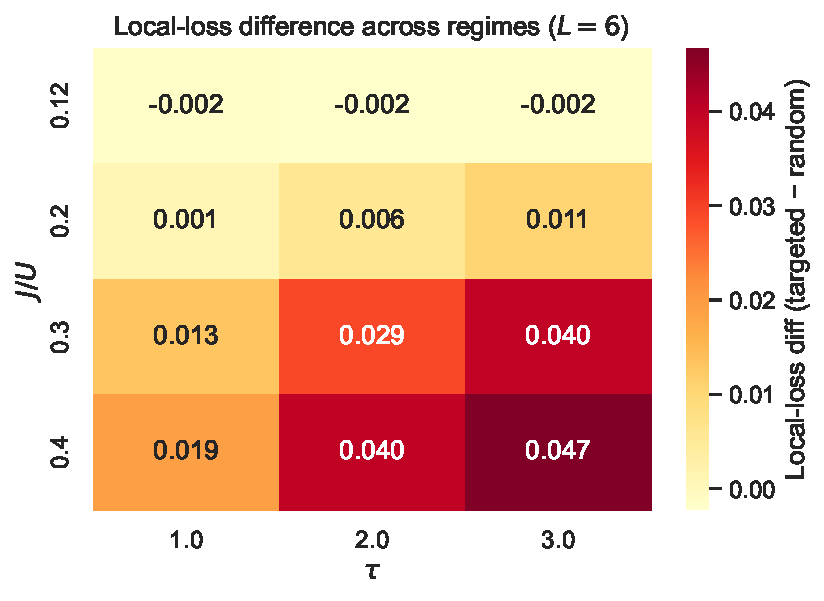
\includegraphics[width=0.85\linewidth]{fig1_main_heatmap.pdf}
\caption{Local-loss difference across $J/U$ and $\tau$ at $L=6$.
The handle effect is positive in the intermediate and stronger coupling
regime and absent or reversed at the lowest tested coupling.}
\label{fig:main_heatmap}
\end{figure}

\subsection{Robustness across chain length}

Table~\ref{tab:robust} shows pooled results at $J/U\in\{0.30,0.40\}$
for $L\in\{6,7\}$.
The positive pocket at $J/U\in\{0.30,0.40\}$ passes at all three tested
chain lengths $L\in\{6,7,8\}$ with 95\% confidence intervals excluding
zero at every horizon $\tau\in\{1,2,3\}$ (Fig.~\ref{fig:robustness}),
confirming that the positive pocket is not a small-size artefact.

The intermediate coupling $J/U=0.20$ is strongly size- and horizon-sensitive,
placing it in the crossover band rather than the robust positive pocket
(see Sec.~\ref{sec:onset}).

\begin{table}[tbp]
\centering
\caption{Pooled local-loss difference for $L\in\{6,7\}$ at
$J/U=0.30$ and $0.40$ (two representative sizes from the full ladder).
Format: mean $[\text{95\% CI}]$, pooling trial-level differences across
$\tau\in\{1,2,3\}$.
All three tested sizes $L\in\{6,7,8\}$ pass at both couplings (see text).}
\label{tab:robust}
\input{outputs/tables/table_robust.tex}
\end{table}

\begin{figure}[tbp]
\centering
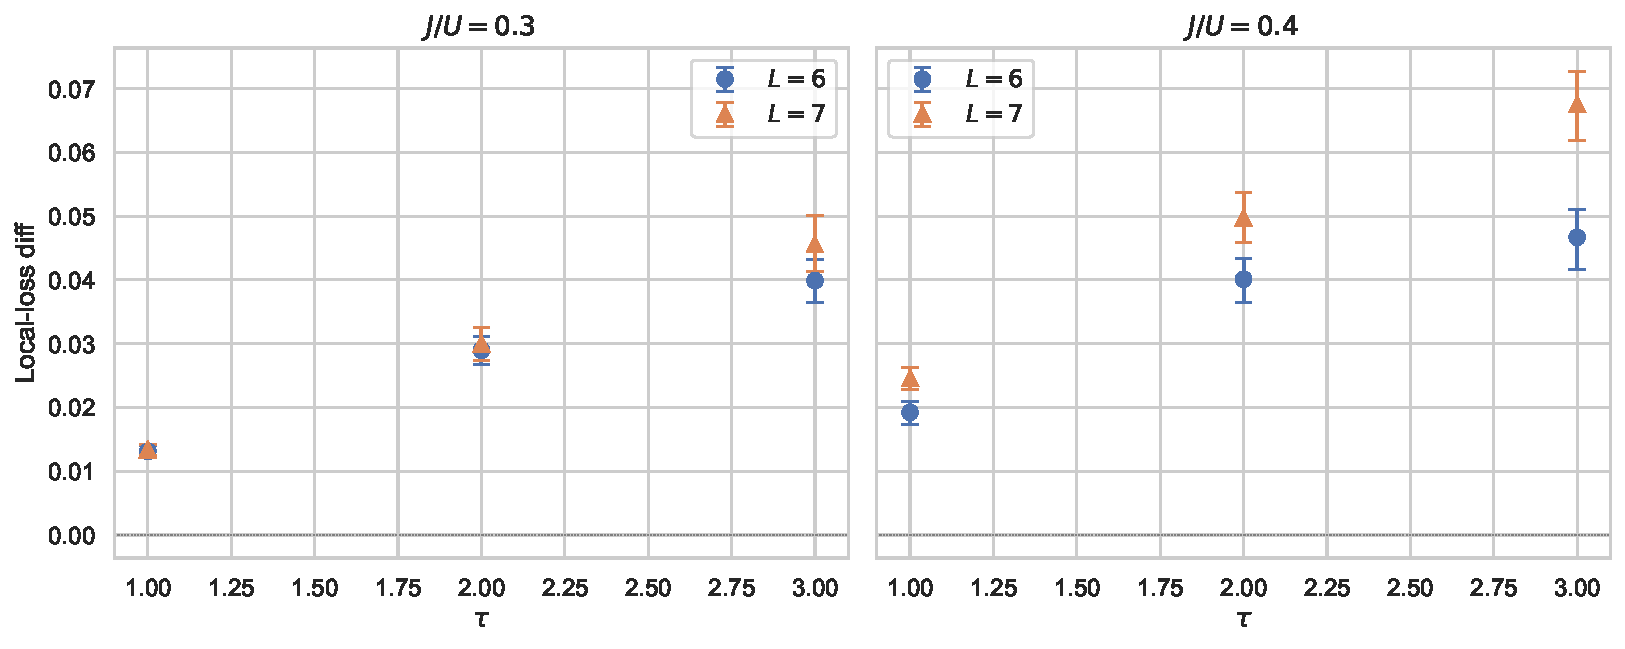
\includegraphics[width=0.85\linewidth]{fig2_robustness.pdf}
\caption{Local-loss difference at $J/U=0.30$ and $0.40$ for
$L=6$ and $L=7$ (two representative sizes). Error bars are 95\% bootstrap CIs.
The same positive result holds at $L=8$; the positive pocket is robust across
all tested $L\in\{6,7,8\}$, with the effect growing with $L$
at the strongest coupling.}
\label{fig:robustness}
\end{figure}

\subsection{Regime map}
\label{sec:regime}

The results define three regimes within the tested parameter range:

\textbf{Low-coupling regime} ($J/U=0.12$):
The targeted intervention produces near-zero to weakly negative responses
relative to random targeting.
In this deep Mott-like regime the occupation-variance handle does not
identify intervention-sensitive sites; the 95\% CIs are below zero at the
paper's burn-in time, but the gaps are small in magnitude and, as shown in
Sec.~\ref{sec:burnin}, partly burn-in-sensitive at $L=6$.

\textbf{Crossover band} ($J/U\approx0.18$--$0.24$, depending on $L$ and $\tau$):
The handle begins to function but its effectiveness is size- and
horizon-dependent.
The first-pass onset shifts upward with $L$ (for fixed $\tau$) and
downward with $\tau$ (for fixed $L$), both trends monotone across the
ladder (see Sec.~\ref{sec:onset}).

\textbf{Positive pocket} ($J/U\gtrsim0.30$):
The handle is consistently positive across all three tested chain lengths
and all horizons $\tau\in\{1,2,3\}$.
This is the regime where the occupation-variance selector reliably
identifies sites whose perturbation produces excess local loss, with CIs
strictly above zero at every tested $(L,\tau)$ combination.

The existence of a negative boundary regime and a structured crossover band
is itself informative: the handle is not a generic property of the dephasing
operator but is sharply regime-dependent.

\subsection{Crossover-band onset}
\label{sec:onset}

Table~\ref{tab:onset} reports the smallest $J/U$ at which the 95\% CI first
strictly excludes zero (first PASS) for $L\in\{6,7,8\}$ and horizons
$\tau\in\{2,3\}$.

\begin{table}[tbp]
\centering
\caption{First-PASS onset coupling: smallest $J/U$ at which the 95\% CI
strictly excludes zero, by chain length $L$ and horizon $\tau$.
Entries $\leq\!0.20$ are bounded by the initial sweep (exact onset lies
in the interval $(0.12,\,0.20]$); entry $>\!0.20$ indicates a failure at
$J/U=0.20$ with onset in $(0.20,\,0.30)$.}
\label{tab:onset}
\begin{ruledtabular}
\begin{tabular}{ccc}
$L$ & $\tau=2$ & $\tau=3$ \\
\colrule
$6$ & $\leq0.20$ & $\leq0.20$ \\
$7$ & $>0.20$    & $\leq0.20$ \\
$8$ & $0.20$     & $0.18$     \\
\end{tabular}
\end{ruledtabular}
\end{table}

The onset coupling is non-decreasing with $L$ for fixed $\tau$,
and non-increasing with $\tau$ for fixed $L$, across the full tested range.
Any coupling $J/U\gtrsim0.30$ lies above the onset for all tested
$(L,\tau)$ combinations, consistently defining the positive pocket boundary.

\subsection{Spatial response pattern}

Fig.~\ref{fig:mechanism} shows the site-resolved occupation change at
$L=6$, $\tau=2$ for both regimes side by side: the low-coupling regime
(panel a, $J/U=0.12$) and the positive pocket (panel b, $J/U=0.30$).
The bars show the mean site-resolved occupation change under the
deterministic targeted intervention and averaged across the 100
matched-budget random interventions.

The positive-pocket panel (b) is consistent with a nonlocal, redistributive
response: under targeted intervention, the selected central sites (shaded)
show less negative occupation change than under random intervention, while
non-selected sites show increased occupation loss, indicating that the
intervention redistributes occupation across the chain rather than simply
amplifying local loss at the targeted sites.
The low-coupling panel (a) shows the regime-dependent contrast directly:
at $J/U=0.12$, the high-$\Fi$ selected sites (2,3) carry near-zero
occupation change, while sites 1 and 4---outside the selected set---carry
the dominant redistribution signal.
Targeting the variance handle therefore perturbs the same structural
degree of freedom in both regimes, but whether that perturbation leads to
net local loss at the selected sites or redistributes occupation in a
non-beneficial direction depends on the coupling strength.

\begin{figure}[tbp]
\centering
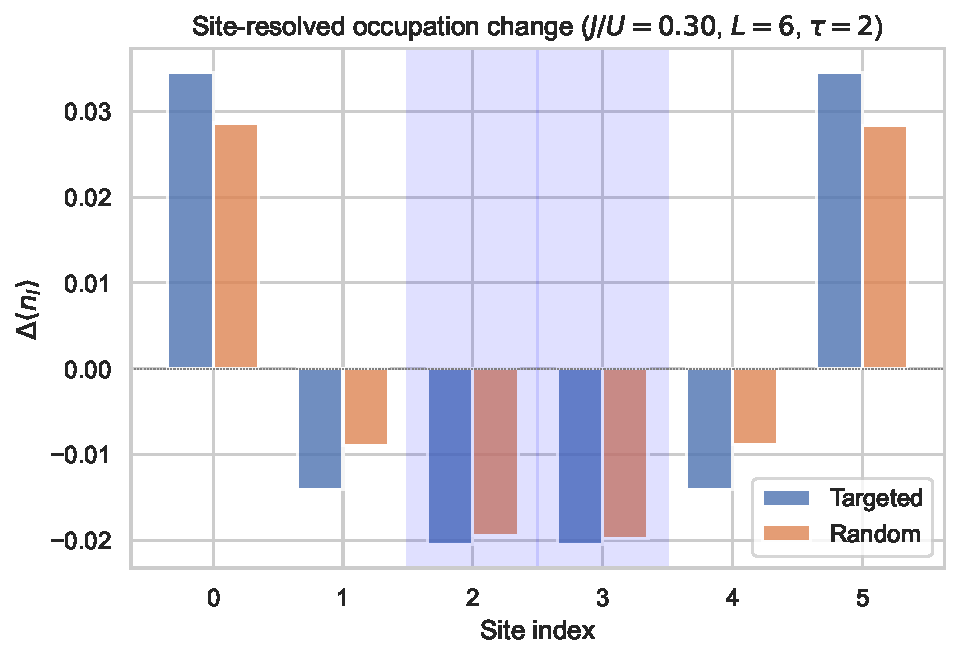
\includegraphics[width=\linewidth]{fig3_mechanism.pdf}
\caption{Mean site-resolved occupation change ($\Delta\langle n_i\rangle$,
$L=6$, $\tau=2$) under targeted versus matched-budget random intervention,
shown for both regimes.
\textbf{(a)} Low-coupling regime ($J/U=0.12$): high-$\Fi$ selected sites
(shaded, sites 2--3) show near-zero response; the large occupation
redistribution occurs at unselected sites 1 and 4, where targeting
provides no advantage.
\textbf{(b)} Positive pocket ($J/U=0.30$): targeted intervention drives
deeper occupation redistribution than random intervention across the
non-selected sites, consistent with the redistribution-handle
interpretation.
Negative values correspond to occupation loss; shaded bands mark selected
sites.}
\label{fig:mechanism}
\end{figure}

\subsection{Disorder selector sweep}
\label{sec:selector}

To test whether the advantage of $\Fi$ targeting is specific to variance
information or reducible to geometry, we broke the clean-chain reflection
symmetry by adding random on-site disorder $\mu_i\sim\mathrm{Uniform}(0,\mu_{\max})$
to the chemical potential.
Nine selectors were compared at $L=6$, 50 disorder realizations, and
$J/U=0.40$, $\tau=3$.
Their definitions are given in Table~\ref{tab:selectors}.

\begin{table}[tbp]
\centering
\caption{Selector definitions used in the disorder sweep.
Each selector picks the top-$k$ (or bottom-$k$) sites by the listed
criterion evaluated on the post-burn-in state $\rho_t$.}
\label{tab:selectors}
\begin{ruledtabular}
\begin{tabular}{ll}
Selector & Definition \\
\hline
fi        & Top-$k$ by $\Fi=\langle\nop_i^2\rangle-\langle\nop_i\rangle^2$ \\
geo       & $k$ sites nearest the chain centre \\
maxn      & Top-$k$ by $\langle\nop_i\rangle$ \\
minn      & Bottom-$k$ by $\langle\nop_i\rangle$ \\
bdy       & $k$ outermost (boundary) sites \\
anti      & Bottom-$k$ by $\Fi$ \\
gen       & Top-$k$ by $|\langle[\hat{L}_i,\hat{H}]\rangle|$, generator action \\
dis\_amp  & Top-$k$ by $|\mu_i|$, disorder amplitude \\
dis\_anti & Bottom-$k$ by $|\mu_i|$ \\
\end{tabular}
\end{ruledtabular}
\end{table}

At strong disorder ($\mu_{\max}\geq1.0$) fi is the top selector
(Fig.~\ref{fig:selector_shellperm}, left):
fi$=+0.049$, maxn$=+0.034$, geo$=+0.032$, gen$=+0.028$,
dis\_amp$=+0.023$, bdy$=+0.010$, dis\_anti$=+0.005$, anti$=+0.002$,
minn$\approx0$.
The fi--geo gap grows monotonically with both $\mu_{\max}$ and $J/U$,
from $+0.0002$ at $\mu_{\max}=0.5$ to $+0.017$ at $\mu_{\max}=2.0$.
The fact that dis\_amp ranks well below fi confirms that $\Fi$ carries
information beyond raw disorder amplitude: variance tracks local
susceptibility to dephasing, not merely where disorder is strongest.
At weak disorder ($\mu_{\max}\lesssim0.5$), symmetry is approximately intact
and fi$\approx$geo, consistent with the clean-chain result.

\subsection{Shell-matched permutation controls}
\label{sec:shellperm}

In the disordered chain, sites can be grouped into shells by their
distance from the nearest boundary.
Shell-matched permutation controls hold shell membership fixed and randomly
permute the assignment of sites within each shell, then apply targeted
dephasing to the permuted top-$k$ sites.
This isolates the within-shell variance information from the shell-level
geometry.

At $L=6$, $\mu_{\max}\leq0.3$, $J/U\geq0.30$, $\tau=3$, fi beats all
shell-matched permutations by $+0.002$ to $+0.006$
(Fig.~\ref{fig:selector_shellperm}, right).
This establishes that $\Fi$ carries within-shell information that is not
captured by shell geometry alone: sites sharing the same shell distance
are not interchangeable when selected by variance.

\subsection{Deterministic inhomogeneous chain}
\label{sec:inhomogeneous}

To test the geometry--variance separation without stochasticity, we
studied a deterministic tilt chain in which a linearly varying chemical
potential $\mu_i = \mu_0(i - (L-1)/2)$ is applied, explicitly breaking
reflection symmetry by design.
The resulting $\Fi$ profile does not peak at the geometric center, so fi
and geo select different sites (overlap zero).

At $J/U=0.40$, $\tau=3$: $\Fi > \mathrm{geo}$ with a gap of $+0.032$ to $+0.054$
(Fig.~\ref{fig:tilt_gammascan}, left).
This non-random, symmetry-breaking control confirms that variance tracks
local number fluctuation structure rather than spatial position, and that
the handle is not simply a proxy for geometric centrality.

\begin{figure}[tbp]
\centering
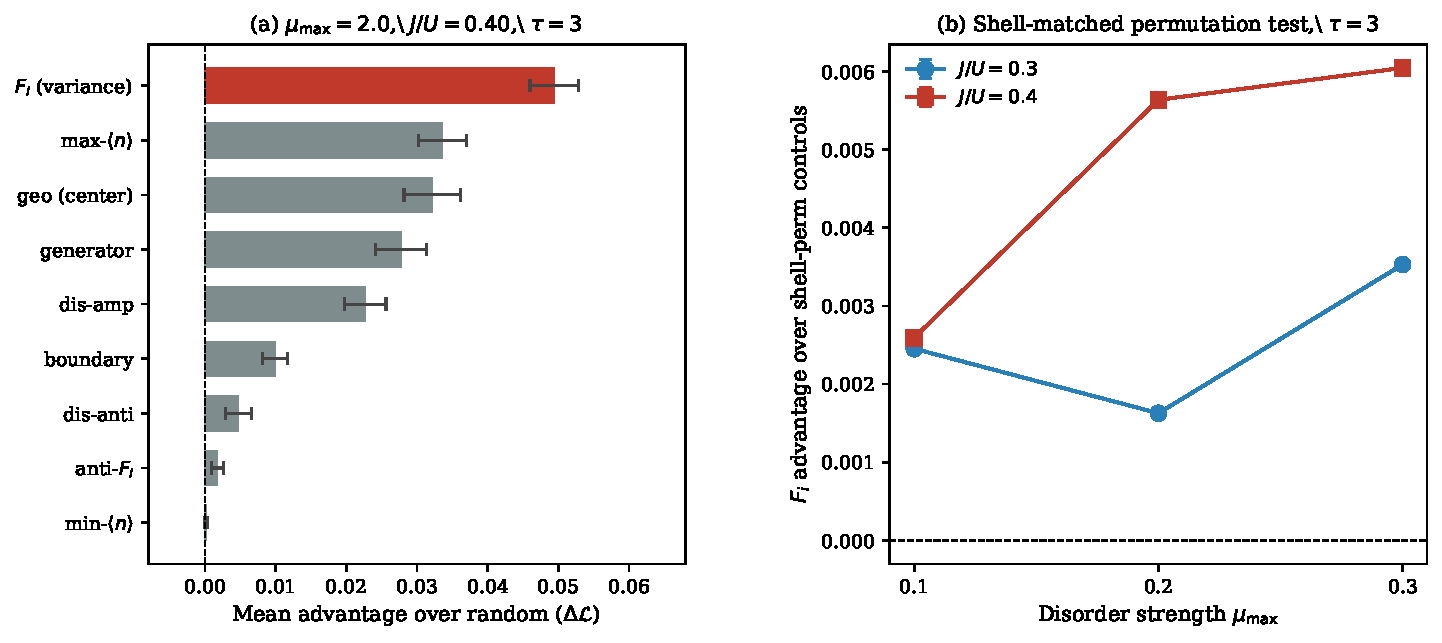
\includegraphics[width=\linewidth]{fig4_selector_shellperm.pdf}
\caption{Selector discrimination under symmetry breaking.
\textbf{Left:} under strong disorder, the variance-based selector $\Fi$
ranks above the tested alternatives, including geometric centrality and
disorder amplitude.
\textbf{Right:} shell-matched permutation controls show that $\Fi$ retains
an advantage beyond shell position alone.
Together these results show that strong disorder separates variance
information from geometry and that the surviving advantage is not reducible
to shell membership.}
\label{fig:selector_shellperm}
\end{figure}

\subsection{Extra dephasing rate scan}
\label{sec:gammascan}

To assess sensitivity to the choice of $\gamma_{\mathrm{extra}}$, we
scanned $\gamma_{\mathrm{extra}}\in\{0.1,0.2,0.5,1.0,2.0\}$ at $L=6$,
$J/U=0.40$, $\tau=3$.
The mean advantages are $+0.0063$, $+0.0106$, $+0.0163$, $+0.0149$,
$+0.0035$ respectively.
The advantage peaks near $\gamma_{\mathrm{extra}}=0.5$--$1.0$ and
collapses at very high rates, where the extra dephasing saturates the
dynamics (Fig.~\ref{fig:tilt_gammascan}, right).
The paper's primary choice $\gamma_{\mathrm{extra}}=0.5$ lies at the
near-optimal point rather than at an arbitrary or cherry-picked value.

\begin{figure}[tbp]
\centering
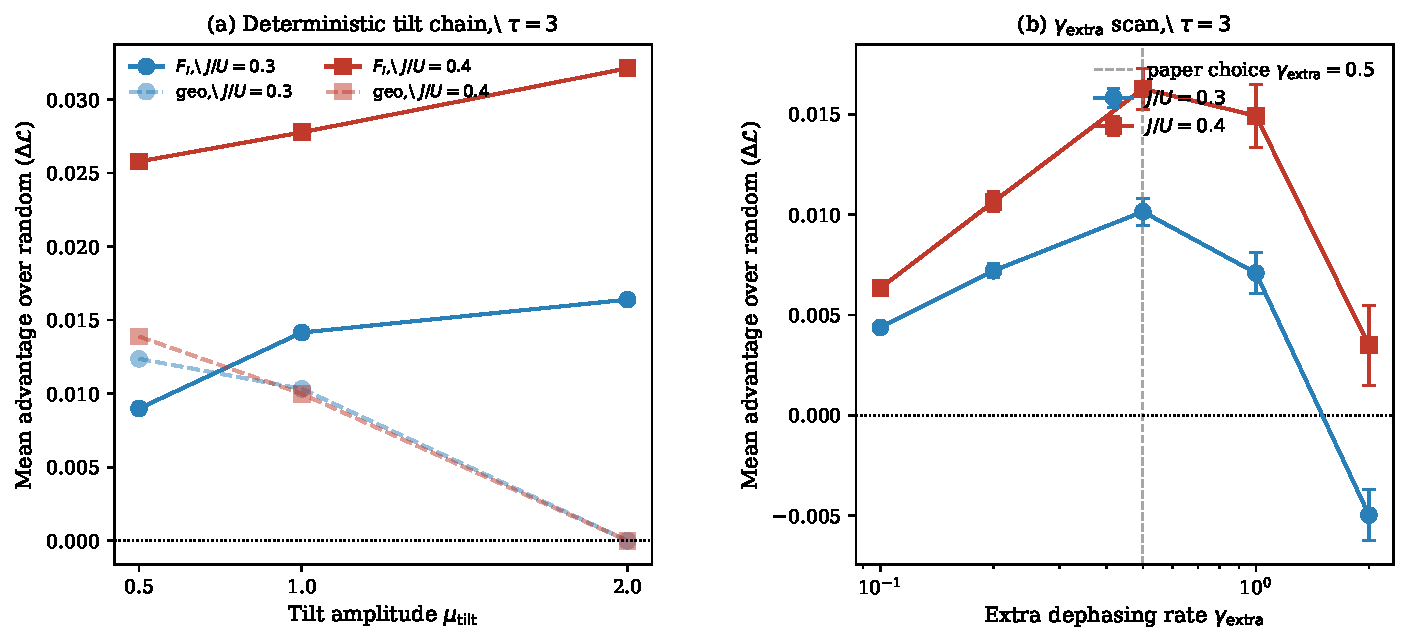
\includegraphics[width=\linewidth]{fig5_tilt_gammascan.pdf}
\caption{Symmetry breaking and intervention-strength robustness.
\textbf{Left:} in a deterministic tilted chain where the variance and
geometric selectors differ by construction, the variance-based selector
outperforms geometric centrality.
\textbf{Right:} the intervention advantage is robust across a broad
mid-range of extra dephasing strength and is near-optimal around
$\gamma_{\mathrm{extra}}\approx0.5$--$1.0$, showing that the main paper
choice is not a tuning artefact.}
\label{fig:tilt_gammascan}
\end{figure}

\subsection{Exhaustive subset ranking and target robustness}
\label{sec:exhaustive}

The comparison against 100 sampled random controls establishes that
the $\Fi$-selected subset outperforms a matched-budget random baseline,
but does not bound its rank among \emph{all} possible subsets.
Because the Hilbert spaces studied here are small enough for exhaustive
enumeration, we evaluated every $\binom{L}{k}$ possible $k$-site subset
($k=\lceil L/3\rceil$; $\binom{6}{2}=15$, $\binom{7}{3}=35$,
$\binom{8}{3}=56$ subsets) under the paper's exact Lindblad protocol,
and ranked the $\Fi$-selected subset by its clipped local-loss percentile.

\begin{table}[tbp]
\centering
\caption{Percentile rank of the $\Fi$-selected subset among all
$\binom{L}{k}$ intervention subsets, clipped local-loss metric.
100 = globally optimal (tied or unique).}
\label{tab:exhaustive}
\begin{ruledtabular}
\begin{tabular}{llrrr}
$L$ & $J/U$ & $\tau=1$ & $\tau=2$ & $\tau=3$ \\
\hline
6 & 0.30 & 100 & 100 & 100 \\
6 & 0.40 & 100 & 100 & 100 \\
7 & 0.30 & 100 & 100 & 100 \\
7 & 0.40 & 100 & 100 & 100 \\
8 & 0.30 & 100 & 100 & 100 \\
8 & 0.40 &  98 &  98 &  98 \\
\hline
6 & 0.20 &  80 &  87 &  87 \\
7 & 0.20 &  29 &  46 &  66 \\
8 & 0.20 &  34 &  68 &  71 \\
\hline
6 & 0.12 &  40 &  40 &  40 \\
7 & 0.12 &  29 &  29 &  29 \\
8 & 0.12 &  21 &  21 &  21 \\
\end{tabular}
\end{ruledtabular}
\end{table}

Table~\ref{tab:exhaustive} reports the results.
In the positive-pocket regime ($J/U\geq0.30$), the $\Fi$-selected subset
is globally optimal or tied for optimal in all $L\in\{6,7\}$ conditions
and at $L=8$, $J/U=0.30$, and remains in the 98th percentile at
$L=8$, $J/U=0.40$ (one of 56 subsets ties or exceeds it).
The crossover band ($J/U=0.20$) yields 29--87th percentile depending on
$L$ and $\tau$, consistent with the regime's size- and horizon-sensitive
character.
The low-coupling regime ($J/U=0.12$) gives 21--40th percentile---the
$\Fi$-selected subset actively ranks below the median, consistent with
the low-coupling-regime result.

We also verified that the positive-pocket advantage is not produced by
the positive-part clipping in the target metric.
For every $(L,\tau)$ condition with $J/U\geq0.30$: the signed local-change
gap (no clipping floor) is positive and exceeds the clipped gap; the
absolute local-change gap is positive; and the global redistribution gap
$\sum_j|\langle\nop_j\rangle_{\mathrm{targeted}}-\langle\nop_j\rangle_{\mathrm{baseline}}|$
is positive.
The clipping is conservative, not inflating: removing it yields a
\emph{larger} advantage in every tested positive-pocket condition.

\subsection{Burn-in sensitivity}
\label{sec:burnin}

Table~\ref{tab:burnin} reports the clipped local-loss gap and exhaustive
subset percentile at $\tau=3$ for three burn-in multipliers ($0.5\times$,
$1.0\times$, $2.0\times$ the paper's baseline $t_{\mathrm{burn}}=5$).
The positive-pocket conclusion ($J/U=0.40$) is stable at both $L=6$ and
$L=8$: the gap remains positive and the $\Fi$-selected subset stays in
the top quartile or above across all three burn-in times.
The low-coupling response ($J/U=0.12$) is much smaller in magnitude
($|\text{gap}|\lesssim0.006$) and partly burn-in-sensitive at $L=6$.
The positive-pocket conclusion is stable under $0.5\times$--$2\times$
burn-in variation at both $L=6$ and $L=8$; the low-coupling response is
much smaller in magnitude and can become burn-in-sensitive at $L=6$.

\begin{table}[tbp]
\centering
\caption{Burn-in sensitivity at $\tau=3$: clipped local-loss gap and
exhaustive-subset percentile at three burn-in multipliers relative to
$t_{\mathrm{burn}}=5$.
Positive gap means the $\Fi$-selected subset exceeds the all-subset mean.}
\label{tab:burnin}
\begin{ruledtabular}
\begin{tabular}{llrrrrr}
$L$ & $J/U$ & $0.5\times$ gap & $1.0\times$ gap & $2.0\times$ gap & Pct.\ range & Sign stable \\
\hline
6 & 0.12 & $-0.002$ & $-0.002$ & $+0.003$ & 40--80\% & no \\
6 & 0.40 & $+0.064$ & $+0.047$ & $+0.012$ & 87--100\% & yes \\
8 & 0.12 & $-0.005$ & $-0.006$ & $<0.001$ & 21--54\% & yes \\
8 & 0.40 & $+0.065$ & $+0.073$ & $+0.009$ & 80--100\% & yes \\
\end{tabular}
\end{ruledtabular}
\end{table}

\subsection{Susceptibility structure: redistribution, not local depletion}
\label{sec:susceptibility}

To probe whether $\Fi$ is grounded in the actual per-site dephasing response,
we compute finite-difference susceptibilities at each site $i$ under a small
extra dephasing dose $\delta\gamma=0.1$:
\begin{align}
\chi^{\mathrm{clip}}_i(\tau)   &= \frac{\max(0,\,\langle\nop_i\rangle_0^\tau - \langle\nop_i\rangle_{\delta\gamma_i}^\tau)}{\delta\gamma}, \\
\chi^{\mathrm{redist}}_i(\tau) &= \frac{\sum_j|\langle\nop_j\rangle_{\delta\gamma_i}^\tau - \langle\nop_j\rangle_0^\tau|}{\delta\gamma},
\end{align}
where $\langle\nop_j\rangle_{\delta\gamma_i}^\tau$ is the occupation at site
$j$ after evolving to horizon $\tau$ with extra dephasing $\delta\gamma$
applied only at site $i$, and $\langle\nop_j\rangle_0^\tau$ is the
corresponding baseline (no extra dephasing).

The Spearman correlation between $\Fi$ and these susceptibilities, computed
over all $L$ sites for each $(L,J/U,\tau)$ condition, reveals a clear
structural distinction. The sign pattern is stable across finite-difference
doses $\delta\gamma\in\{0.05,0.1,0.2\}$.
$\Fi$ is \emph{not} a local-depletion susceptibility: Spearman$(\Fi,
\chi^{\mathrm{clip}})$ is negative at $\tau=1,2$ in nearly all conditions
and only weakly positive at $\tau=3$ in the positive pocket.
By contrast, $\Fi$ is consistently a \emph{redistribution} susceptibility:
Spearman$(\Fi, \chi^{\mathrm{redist}})$ is positive across all regimes and
all $\tau$, reaching values of $0.5$--$1.0$ at $\tau\geq2$ (Fig.~\ref{fig:susc}).
At $L=6$, $\tau\geq2$, the top-$k$ overlap between the highest-$\Fi$ sites
and the highest-$\chi^{\mathrm{redist}}$ sites is $1.0$ in all tested conditions,
meaning $\Fi$ exactly identifies the sites that most strongly perturb the global
occupation distribution per unit extra dephasing.

\begin{figure}[tbp]
\centering

\includegraphics[width=\linewidth]{fig_susceptibility_scatter.pdf}
\caption{Per-site susceptibility vs $\Fi$ at $\tau=3$ for representative
conditions.
\textbf{Top row:} redistribution susceptibility
$\chi^{\mathrm{redist}}_i$ vs $\Fi$ --- Spearman correlation is positive
in all four panels.
\textbf{Bottom row:} local-depletion susceptibility
$\chi^{\mathrm{clip}}_i$ vs $\Fi$ --- correlation is negative or near zero
in three of four panels, and weakly positive only at $J/U=0.40$.
The contrast establishes that $\Fi$ is a redistribution handle, not a
local-depletion handle.}
\label{fig:susc}
\end{figure}

This susceptibility structure provides a mechanistic interpretation of
the regime-dependence: $\Fi$ consistently identifies sites with high
redistribution susceptibility, but whether that redistribution leads to
net local occupation loss at the selected sites (positive pocket) or net
local gain (negative regime) depends on the global response pattern at
that coupling strength.
The variance handle works not by directly depleting targeted sites but by
controlling how occupation is redistributed across the chain on the
time scale $\tau$.

\section{Predictive observability and intervention leverage point at different sites}
\label{sec:t1}

The intervention protocol of Sec.~\ref{sec:results} answers two
distinct questions about each site $i$:
(i) does the pre-intervention local pattern at site $i$ predict the
system's response to a generic dephasing perturbation?
(ii) does targeting site $i$ produce a measurably larger advantage over
matched-budget random targeting than other sites?
The first question concerns predictive observability of a future
response; the second concerns the causal effectiveness of selecting that
specific site. The two questions need not have the same answer.
This section tests whether they agree across the available
$52$ saved $(L, J/U, \tau)$ cells.

\subsection{Observable family and per-cell predictive/causal scores}

Twelve site-resolved observables are grouped into three classes by
physical content.
The \emph{variance class} contains four observables derived from the
pre-intervention $\Fi$ profile: $F_i$, the descending $F$-rank,
$F_i - \overline{F}$, and the per-cell $z$-scored $F_i$.
The \emph{response class} contains five observables derived from the
post-intervention shifts $\Delta\langle\nop_i\rangle$:
$\Delta\langle\nop_i\rangle_{\mathrm{tgt}}$, the trial-mean random-arm
response $\overline{\Delta\langle\nop_i\rangle_{\mathrm{rnd}}}$, their
absolute values, and the redistribution-clipped target
$\max\bigl(0,-\Delta\langle\nop_i\rangle_{\mathrm{tgt}}\bigr)$ used as
the primary metric in Sec.~\ref{sec:primary}.
The \emph{gap class} contains three observables comparing the targeted
and random arms per site: $|\Delta\langle\nop_i\rangle_{\mathrm{tgt}}|
- \overline{|\Delta\langle\nop_i\rangle_{\mathrm{rnd}}|}$, its signed
analogue, and the redistribution gap.

For each cell $c=(L,J/U,\tau)$ and each observable $X$ in the family,
the \emph{predictive score} is the absolute Pearson correlation across
sites between $X_i$ and the trial-mean random-arm response pattern.
The \emph{predictive winner} $X^{\star}(c)$ is the observable maximizing
this score; the \emph{predicted-best site} is
$i^{\mathrm{pred}}(c) = \arg\max_i X^{\star}(c)_i$.
The \emph{causal-best site} $i^{\mathrm{caus}}(c)$ is the site of
largest per-site advantage of targeting,
\begin{equation}
i^{\mathrm{caus}}(c) = \arg\max_i\;\bigl(
  |\Delta\langle\nop_i\rangle_{\mathrm{tgt}}|
  - \overline{|\Delta\langle\nop_i\rangle_{\mathrm{rnd}}|}\bigr).
\end{equation}
The cell is \emph{dissociated} if $i^{\mathrm{pred}}(c)\neq
i^{\mathrm{caus}}(c)$.

\subsection{Dissociation rate}

Across all 52 cells the dissociation rate is $0.904$ ($47/52$).
The pre-intervention site whose pattern best predicts the random-arm
response is the same as the site of largest causal advantage in only $5$
of $52$ conditions.
Replacing the predictive target with the deterministic targeted-arm
response pattern, as a sensitivity check, gives a dissociation rate of
$0.538$, still above the pre-registered $0.50$ threshold but markedly
weaker.
The pre-registered alternative hypothesis (predictive and causal sites
agree in $\geq 80\%$ of cells) is rejected.

\subsection{Reading}

The two questions the protocol asks of the data---``where do we see the
system's variability most predictively?'' and ``where do we get the
most leverage from targeted intervention?''---have different answers
in $90\%$ of conditions.
This is the structural correlate of the choice in
Sec.~\ref{sec:methods} to define the redistribution handle through an
explicit interventional comparison rather than through predictive
correlation alone: the two channels are operationally distinct in this
system, and a definition that tracks one would not in general track the
other.

\section{Structural correlate of the regime boundary at $L=8$}
\label{sec:t3}

The sweeps in Sec.~\ref{sec:primary} establish an empirical regime
boundary near $J/U\approx 0.30$: below this value the $\Fi$ selector is
near-zero or weakly harmful, above it the selector is robustly
beneficial.
This section asks whether the boundary corresponds to a sharp
reorientation of the per-site response pattern as $J/U$ varies.

\subsection{Principal direction of the response}

For each cell $(L, J/U, \tau)$ the per-site gap profile
\begin{equation}
g_i(L,J/U,\tau) = |\Delta\langle\nop_i\rangle_{\mathrm{tgt}}|
  - \overline{|\Delta\langle\nop_i\rangle_{\mathrm{rnd}}|}
\end{equation}
defines a unit direction in site space,
$\hat g(L,J/U,\tau) = g/\|g\|$.
Two adjacent $J/U$ values yield a principal-direction angle
\begin{equation}
\label{eq:thetajj}
\theta_{j\to j+1} = \arccos\bigl|\langle\hat g_j,\hat g_{j+1}\rangle\bigr|,
\end{equation}
where the absolute value handles the sign-ambiguity of unit directions
recovered by SVD.

\subsection{Direction reorientation at $J/U\approx 0.30$, $L=8$}

For $L=8$ at $\tau=2$ the consecutive-$J/U$ angles
[Eq.~\eqref{eq:thetajj}] across the data are, ordered by lower endpoint
$J/U\in\{0.16,0.18,0.20,0.22,0.24,0.26,0.28\}$,
\begin{equation}
(\theta_{1\to 2},\dots,\theta_{7\to 8}) =
(1.02, 0.95, 0.88, 0.28, 1.04, 1.12, \mathbf{1.28})\;\text{rad}.
\end{equation}
The maximum, $1.28$ rad, occurs at the pair $(0.28, 0.30)$ that
straddles the empirical regime boundary.
The principal direction of the intervention response in site space
reorients sharply across this pair.
At $\tau=3$ the maximum angle is $1.48$ rad on the pair $(0.26, 0.28)$,
also inside the locked threshold band $[0.24, 0.32]$.
Compared to the median consecutive-pair angle of $0.91$ rad outside the
band, the threshold reorientation is $1.40\times$ at $\tau=2$.

The signal sharpens substantially under the redistribution-gap
observable
$g^{\mathrm{redist}}_i = \max(0,-\Delta\langle\nop_i\rangle_{\mathrm{tgt}})
- \overline{\max(0,-\Delta\langle\nop_i\rangle_{\mathrm{rnd}})}$,
which mirrors the original paper's primary clipped target
[Eq.~\eqref{eq:target}].
Under this observable the threshold pair $(0.28, 0.30)$ at $L=8$,
$\tau=2$ produces an angle of $1.11$ rad against an off-band median of
$0.34$ rad, a ratio of $\mathbf{3.25\times}$.
The structural reorientation co-localized with the empirical regime
boundary is unambiguous under the metric closest to the original
paper's target definition.

\subsection{Size dependence}

At $L=9$ the consecutive-$J/U$ angle sequence does not show a sharp
peak in the threshold band: the largest shift sits at the pair
$(0.30, 0.40)$, outside the locked band, and the in-band maximum is
below the off-band median.
This is true under both the primary gap observable and the
redistribution-gap observable.
The structural correlate of the regime boundary is therefore a feature
visible at $L=8$ but not at $L=9$ within the available simulations.

The discrepancy admits at least three readings.
First, the $L=9$ data includes the additional $J/U=0.40$ point that the
$L=8$ sweep does not, and this larger value may dominate the
finite-sweep response geometry by exposing a different feature of the
dynamics.
Second, the finite-size threshold may shift to a different $J/U$ at
$L=9$, manifesting as the larger angle on the $(0.30, 0.40)$ pair.
Third, the structural reorientation may be specific to the regime where
finite-size effects are weakest.
The available data does not discriminate between these readings.
The structural explanation in this section is reported as $L=8$
specific.

\section{Additional structural findings}
\label{sec:t246}

This section reports three further structural results from the same
data: a clustering of observables by physical class, a
thermalization-driven convergence of observables across the Lindblad
horizon, and a disagreement among three natural single-site scoring
rules.
A subsection on pre-registered failures and not-testable predictions
closes the section.

\subsection{Subspace clustering of observables by class}
\label{sec:t2}

For each $L\in\{6,8,9\}$ and each of the 12 observables defined in
Sec.~\ref{sec:t1} we form the cell-by-site matrix $M_X[c,i] = X_i$ at
cell $c$, $z$-scored within each cell.
The top-$r=2$ right-singular subspace of $M_X$ in $\mathbb{R}^L$ is the
two-dimensional plane that captures the observable's dominant
cell-to-cell variation in site space.
For each pair of observables we compute the larger of the two principal
angles between their planes.

The 12 observables fall into three classes (variance, response, gap)
giving $\binom{4}{2}+\binom{5}{2}+\binom{3}{2}=19$ same-class pairs and
$47$ cross-class pairs (66 pairs in total per $L$).
At every tested $L$ the median same-class principal angle is strictly
less than the median cross-class angle:
$0.028$ rad versus $0.060$ rad at $L=6$,
$1.31$ rad versus $1.53$ rad at $L=8$,
$0.38$ rad versus $0.97$ rad at $L=9$.
The empirical pairwise angle distribution differs from a uniform-on-
Stiefel (Haar) null at $p < 10^{-5}$ via two-sample Kolmogorov--Smirnov
at every $L$, with the empirical distribution showing a longer left
tail (lower 25th percentile) than the null in every case.
Same-class observables cluster more tightly in subspace alignment than
would arise by chance.

The qualitative ordering (within $<$ across, KS-distinguishable from
random) holds at every $L$.
The absolute medians do not transfer cleanly across $L$ because the
ambient site space is small ($L\leq 9$) and finite-size compression
either pushes the entire distribution near zero (at $L=6$) or near
$\pi/2$ (at $L=8$); see Sec.~\ref{sec:scope_t} for the
pre-registered numerical-magnitude prediction this compression breaks.

\subsection{Observable convergence across the Lindblad horizon}
\label{sec:t4}

The same observable family at multiple $\tau$ values within a fixed $L$
yields a coarse temporal picture of how the structural distinctions
between observable classes evolve.
At $L=6$, where the data covers $\tau\in\{1,2,3\}$, the median pairwise
principal angle decreases monotonically from $1.40$ rad at $\tau=1$ to
$0.27$ rad at $\tau=2$ to $0.18$ rad at $\tau=3$.
At later horizons the observables converge toward a common subspace:
the structural distinctions between variance-, response-, and gap-class
observables fade as the chain approaches its dissipative steady state.
At $L=8$ the available pair $\tau\in\{2,3\}$ shows $1.40\to 1.39$ rad
(weak shrinkage).
At $L=9$ the corresponding pair shows $0.76\to 0.65$ rad; restricted to
the four $J/U$ values where $L=9$ also stores $\tau=1$, the three-point
sequence is $1.06\to 0.82\to 0.65$ rad.
At every tested $L$ the median angle is non-increasing in $\tau$,
consistent with continuous Lindblad-driven loss of structure in the
observable family as the system thermalizes.

\subsection{Three single-site scoring rules disagree on the optimal site}
\label{sec:t5}

Three natural scoring rules suggest themselves for ranking single-site
interventions retrospectively from the random-arm trials.
A \emph{trace} rule scores a site by the average total movement
$\sum_j |\Delta\langle\nop_j\rangle_{\mathrm{rnd}}|$ across random
trials in which that site was hit.
A \emph{max-response} rule scores a site by the average maximum
single-site movement $\max_j |\Delta\langle\nop_j\rangle_{\mathrm{rnd}}|$
in those trials.
A \emph{gap} rule scores a site by the average advantage of having that
site in the hit set relative to sites left out of it.
The three rules are different operationalizations of ``which single
site is best to target.''

Across all 52 cells the three rules' optimal-site choices are never
unanimous: the all-three-agree rate is $0$.
The pairwise disagreement rates are $1.00$ for trace-versus-gap,
$1.00$ for max-response-versus-gap, and $0.35$ for
trace-versus-max-response.
The choice of scoring rule changes the conclusion in every cell.
This is consistent with, and structurally explains, the choice in
Sec.~\ref{sec:exhaustive} to compare signed, absolute, and
redistribution-clipped target definitions and report all three:
the scoring rule is itself a degree of freedom that no fixed choice can
neutralize.

\subsection{Pre-registered failures and not-testable predictions}
\label{sec:scope_t}

Two pre-registered structural predictions failed and are reported as
failures.

A \emph{magnitude-floor} prediction asserting same-class median
principal angle $< 0.7$ rad and cross-class median $> 1.0$ rad
\emph{at every} $L$ failed at every tested $L$.
The qualitative ordering (within $<$ across, KS distinguishable from
random) is robust per Sec.~\ref{sec:t2}; the locked numerical floor was
calibrated for higher-dimensional ambient spaces and does not transfer
to the $L\leq 9$ chains studied here.
At $L=6$ the entire pairwise distribution is compressed below $0.1$
rad; at $L=8$ it is compressed near $\pi/2$.
The structural-clustering result generalizes; the specific numerical
ranges do not.

A \emph{universal threshold reorientation} prediction asserting that
the principal-direction shift co-localized with the regime boundary
appears at \emph{both} $L=8$ and $L=9$ failed at $L=9$.
The structural correlate is present at $L=8$ but not at $L=9$ within
the available simulations (Sec.~\ref{sec:t3}).

A third pre-registered question---ranking observables by their
susceptibility \emph{across multiple intervention types} (additional
dephasing, particle injection, phase imprinting, local heating)---was
declared not testable on the existing data, since only additional
dephasing was simulated.
Extending the protocol to other intervention channels would require new
simulations and is outside the scope of this paper.

These failures and the not-testable declaration were locked in the
pre-registration before any analysis was run; they are reported as
locked failures, not downgraded to exploratory observations.

\section{Discussion}
\label{sec:disc}

\paragraph*{Summary.}
In the tested one-dimensional open Bose--Hubbard chain, local number
variance $\Fi = \langle\nop_i^2\rangle - \langle\nop_i\rangle^2$
functions as a finite-size, regime-dependent redistribution handle:
in the positive pocket $J/U\geq0.30$, targeting the highest-$\Fi$ sites
with additional dephasing produces more local future occupation loss than
matched-budget random targeting, robustly across all tested $L\in\{6,7,8\}$
and $\tau\in\{1,2,3\}$, with the effect increasing with system size.
Exhaustive enumeration of all $\binom{L}{k}$ intervention subsets
further shows that the $\Fi$-selected subset lies at the top of the
subset-response distribution in the positive pocket, and this advantage
survives signed, absolute, and redistribution-based target definitions.
The handle is regime-dependent---near-zero to weakly harmful at $J/U=0.12$,
transitional near $J/U\approx0.20$---and its advantage is not reducible to
geometric centrality, shell position, mean occupation, or disorder amplitude.

\paragraph*{Mechanism.}
The susceptibility analysis in Sec.~\ref{sec:susceptibility} shows that
$\Fi$ is a redistribution susceptibility rather than a local-depletion
susceptibility: high-$\Fi$ sites are those where a small extra dephasing
dose most strongly perturbs the global occupation pattern.
Whether this redistribution results in net local loss at the targeted sites
(positive pocket) or net local gain (low-coupling regime) depends on the
coupling-strength-dependent global response structure, not on any local
property of the sites themselves.
A full microscopic account of this redistribution---connecting $\Fi$ to the
Lindblad generator spectrum or the Green's function of the superoperator---
is left for future work.

\paragraph*{Structural follow-up.}
The pre-registered analyses in Secs.~\ref{sec:t1}--\ref{sec:t246} add
three structural observations that the empirical sweeps in
Sec.~\ref{sec:results} do not by themselves expose.
First, the site whose pre-intervention $\Fi$ best predicts the
random-arm response disagrees in $90.4\%$ of saved cells with the site
yielding the largest causal advantage of targeting; predictive
observability and intervention leverage are operationally distinct
channels in this system, which is the structural reason the original
paper defines the handle through an explicit interventional contrast
rather than a predictive correlation.
Second, the empirical regime boundary near $J/U\approx 0.30$
co-localizes at $L=8$ with a sharp reorientation of the principal
direction of the per-site response in site space (ratio $3.25\times$
under the redistribution-gap observable), supplying a structural
correlate of the boundary that the original sweeps reported only as an
empirical fact.
Third, observable subspaces converge with the Lindblad horizon
($L=6$ median pairwise principal angle: $1.40$ rad at $\tau=1$,
$0.18$ rad at $\tau=3$), and three natural single-site scoring rules
disagree on the optimal site in $100\%$ of cells---consistent with the
multi-target-definition robustness reported in
Sec.~\ref{sec:exhaustive}.
These structural findings strengthen rather than replace the original
empirical claims; they were locked in a pre-registration document
before any analysis was performed (Sec.~\ref{sec:reanalysis_methods}),
and the locked failures (a universal numerical magnitude floor on
subspace alignment, the threshold reorientation at $L=9$) are reported
as failures bounding the structural reach within the available
simulations.

\paragraph*{What is not claimed.}
The exhaustive enumeration establishes near-optimality within the
finite-size systems studied; we do not claim this extends to the
thermodynamic limit, to all coupling regimes, or to other quantum systems.
No claim is made that $\gamma_{\mathrm{extra}}=0.5$ is a globally
optimal dephasing rate, or that the occupation-variance handle corresponds
to any equilibrium observable.
The observed regime boundary near $J/U\approx0.20$ should not be
identified with the thermodynamic Mott--superfluid transition.
In these small open chains under dissipation it is best interpreted as a
finite-size dynamical crossover in the response of the Lindblad evolution,
not as a sharp equilibrium phase boundary.

\paragraph*{Scope and limitations.}
The Hilbert-space dimension of the fixed-$N$ sector grows combinatorially
with $L$ and $n_{\max}$, limiting exact Lindblad evolution to small chains.
The tested range ($L\leq8$, $n_{\max}=3$) establishes the effect in the
positive pocket but does not access the thermodynamic limit.
Whether the positive pocket persists, broadens, or shifts at larger system
sizes is an open question requiring approximate methods such as
matrix-product-operator Lindblad evolution~\cite{daley2014}.
As a truncation check, we repeated the $L=8$, $N=4$ conditions with
$n_{\max}=4$ (the only tested case where the $n_{\max}=3$ cutoff is active,
$D=322\to330$); the regime ordering, sign pattern, and top-$\Fi$
subset-percentile tier are unchanged across all tested conditions, with
local-loss gap shifts below $2\times10^{-4}$.

\paragraph*{Experimental relevance.}
The 1D open Bose--Hubbard model under dephasing is experimentally
motivated.
Cold-atom optical-lattice platforms already realise 1D Bose--Hubbard-like
systems with tunable $J/U$~\cite{jaksch1998,greiner2002}, and recent
advances in quantum-gas microscopy provide site-resolved preparation and
readout relevant to the targeted-intervention protocol studied
here~\cite{gross2021}.
The Lindblad dephasing modelled by $\gamma\hat{n}_i$ is a standard
approximation for photon-scattering-induced decoherence in optical
lattices~\cite{pichler2010,daley2014}.
The present results therefore constitute a theory-side proposal with
experimental plausibility: the positive-pocket and crossover-band
structures identified here are, in principle, accessible to existing
site-resolved cold-atom platforms, though the exact targeted-dephasing protocol has not yet been implemented
experimentally.

\begin{acknowledgments}
The author thanks the open-source scientific Python community for the
libraries underlying this work: NumPy, SciPy~\cite{scipy2020}, pandas,
matplotlib, and tqdm.
\end{acknowledgments}

\section*{Data and Code Availability}

All simulation code and raw data are available at
\href{https://github.com/kunalb541/BH}{https://github.com/kunalb541/BH}.

\bibliography{refs}

\end{document}
